\documentclass[]{article}
\usepackage{lmodern}
\usepackage{amssymb,amsmath}
\usepackage{ifxetex,ifluatex}
\usepackage{fixltx2e} % provides \textsubscript
\ifnum 0\ifxetex 1\fi\ifluatex 1\fi=0 % if pdftex
  \usepackage[T1]{fontenc}
  \usepackage[utf8]{inputenc}
  \usepackage{eurosym}
\else % if luatex or xelatex
  \ifxetex
    \usepackage{mathspec}
  \else
    \usepackage{fontspec}
  \fi
  \defaultfontfeatures{Ligatures=TeX,Scale=MatchLowercase}
  \newcommand{\euro}{€}
\fi
% use upquote if available, for straight quotes in verbatim environments
\IfFileExists{upquote.sty}{\usepackage{upquote}}{}
% use microtype if available
\IfFileExists{microtype.sty}{%
\usepackage{microtype}
\UseMicrotypeSet[protrusion]{basicmath} % disable protrusion for tt fonts
}{}
\usepackage[margin=1in]{geometry}
\usepackage{hyperref}
\hypersetup{unicode=true,
            pdftitle={SD\_dataset},
            pdfauthor={Katarzyna Otko},
            pdfborder={0 0 0},
            breaklinks=true}
\urlstyle{same}  % don't use monospace font for urls
\usepackage{color}
\usepackage{fancyvrb}
\newcommand{\VerbBar}{|}
\newcommand{\VERB}{\Verb[commandchars=\\\{\}]}
\DefineVerbatimEnvironment{Highlighting}{Verbatim}{commandchars=\\\{\}}
% Add ',fontsize=\small' for more characters per line
\usepackage{framed}
\definecolor{shadecolor}{RGB}{248,248,248}
\newenvironment{Shaded}{\begin{snugshade}}{\end{snugshade}}
\newcommand{\KeywordTok}[1]{\textcolor[rgb]{0.13,0.29,0.53}{\textbf{#1}}}
\newcommand{\DataTypeTok}[1]{\textcolor[rgb]{0.13,0.29,0.53}{#1}}
\newcommand{\DecValTok}[1]{\textcolor[rgb]{0.00,0.00,0.81}{#1}}
\newcommand{\BaseNTok}[1]{\textcolor[rgb]{0.00,0.00,0.81}{#1}}
\newcommand{\FloatTok}[1]{\textcolor[rgb]{0.00,0.00,0.81}{#1}}
\newcommand{\ConstantTok}[1]{\textcolor[rgb]{0.00,0.00,0.00}{#1}}
\newcommand{\CharTok}[1]{\textcolor[rgb]{0.31,0.60,0.02}{#1}}
\newcommand{\SpecialCharTok}[1]{\textcolor[rgb]{0.00,0.00,0.00}{#1}}
\newcommand{\StringTok}[1]{\textcolor[rgb]{0.31,0.60,0.02}{#1}}
\newcommand{\VerbatimStringTok}[1]{\textcolor[rgb]{0.31,0.60,0.02}{#1}}
\newcommand{\SpecialStringTok}[1]{\textcolor[rgb]{0.31,0.60,0.02}{#1}}
\newcommand{\ImportTok}[1]{#1}
\newcommand{\CommentTok}[1]{\textcolor[rgb]{0.56,0.35,0.01}{\textit{#1}}}
\newcommand{\DocumentationTok}[1]{\textcolor[rgb]{0.56,0.35,0.01}{\textbf{\textit{#1}}}}
\newcommand{\AnnotationTok}[1]{\textcolor[rgb]{0.56,0.35,0.01}{\textbf{\textit{#1}}}}
\newcommand{\CommentVarTok}[1]{\textcolor[rgb]{0.56,0.35,0.01}{\textbf{\textit{#1}}}}
\newcommand{\OtherTok}[1]{\textcolor[rgb]{0.56,0.35,0.01}{#1}}
\newcommand{\FunctionTok}[1]{\textcolor[rgb]{0.00,0.00,0.00}{#1}}
\newcommand{\VariableTok}[1]{\textcolor[rgb]{0.00,0.00,0.00}{#1}}
\newcommand{\ControlFlowTok}[1]{\textcolor[rgb]{0.13,0.29,0.53}{\textbf{#1}}}
\newcommand{\OperatorTok}[1]{\textcolor[rgb]{0.81,0.36,0.00}{\textbf{#1}}}
\newcommand{\BuiltInTok}[1]{#1}
\newcommand{\ExtensionTok}[1]{#1}
\newcommand{\PreprocessorTok}[1]{\textcolor[rgb]{0.56,0.35,0.01}{\textit{#1}}}
\newcommand{\AttributeTok}[1]{\textcolor[rgb]{0.77,0.63,0.00}{#1}}
\newcommand{\RegionMarkerTok}[1]{#1}
\newcommand{\InformationTok}[1]{\textcolor[rgb]{0.56,0.35,0.01}{\textbf{\textit{#1}}}}
\newcommand{\WarningTok}[1]{\textcolor[rgb]{0.56,0.35,0.01}{\textbf{\textit{#1}}}}
\newcommand{\AlertTok}[1]{\textcolor[rgb]{0.94,0.16,0.16}{#1}}
\newcommand{\ErrorTok}[1]{\textcolor[rgb]{0.64,0.00,0.00}{\textbf{#1}}}
\newcommand{\NormalTok}[1]{#1}
\usepackage{graphicx,grffile}
\makeatletter
\def\maxwidth{\ifdim\Gin@nat@width>\linewidth\linewidth\else\Gin@nat@width\fi}
\def\maxheight{\ifdim\Gin@nat@height>\textheight\textheight\else\Gin@nat@height\fi}
\makeatother
% Scale images if necessary, so that they will not overflow the page
% margins by default, and it is still possible to overwrite the defaults
% using explicit options in \includegraphics[width, height, ...]{}
\setkeys{Gin}{width=\maxwidth,height=\maxheight,keepaspectratio}
\IfFileExists{parskip.sty}{%
\usepackage{parskip}
}{% else
\setlength{\parindent}{0pt}
\setlength{\parskip}{6pt plus 2pt minus 1pt}
}
\setlength{\emergencystretch}{3em}  % prevent overfull lines
\providecommand{\tightlist}{%
  \setlength{\itemsep}{0pt}\setlength{\parskip}{0pt}}
\setcounter{secnumdepth}{0}
% Redefines (sub)paragraphs to behave more like sections
\ifx\paragraph\undefined\else
\let\oldparagraph\paragraph
\renewcommand{\paragraph}[1]{\oldparagraph{#1}\mbox{}}
\fi
\ifx\subparagraph\undefined\else
\let\oldsubparagraph\subparagraph
\renewcommand{\subparagraph}[1]{\oldsubparagraph{#1}\mbox{}}
\fi

%%% Use protect on footnotes to avoid problems with footnotes in titles
\let\rmarkdownfootnote\footnote%
\def\footnote{\protect\rmarkdownfootnote}

%%% Change title format to be more compact
\usepackage{titling}

% Create subtitle command for use in maketitle
\newcommand{\subtitle}[1]{
  \posttitle{
    \begin{center}\large#1\end{center}
    }
}

\setlength{\droptitle}{-2em}

  \title{SD\_dataset}
    \pretitle{\vspace{\droptitle}\centering\huge}
  \posttitle{\par}
    \author{Katarzyna Otko}
    \preauthor{\centering\large\emph}
  \postauthor{\par}
      \predate{\centering\large\emph}
  \postdate{\par}
    \date{4 wrzeÄąâ\euro{}şnia 2020}


\begin{document}
\maketitle

Some text

\begin{Shaded}
\begin{Highlighting}[]
\KeywordTok{library}\NormalTok{(dplyr)}
\KeywordTok{library}\NormalTok{(ggplot2)}
\KeywordTok{library}\NormalTok{(reshape2)}
\KeywordTok{setwd}\NormalTok{(}\StringTok{'C:/Users/katin/Desktop/Folder/STUDIA/DTU/Semestr I/Intro to ML/Project I'}\NormalTok{)}
\NormalTok{SD <-}\StringTok{ }\KeywordTok{read.csv}\NormalTok{(}\StringTok{'Speed Dating Data.csv'}\NormalTok{)}

\CommentTok{# numdim(SDber of rows and columns}
\KeywordTok{dim}\NormalTok{(SD)}
\end{Highlighting}
\end{Shaded}

\begin{verbatim}
## [1] 8378  195
\end{verbatim}

\begin{Shaded}
\begin{Highlighting}[]
\CommentTok{# number of women}
\KeywordTok{length}\NormalTok{(}\KeywordTok{unique}\NormalTok{(SD}\OperatorTok{$}\NormalTok{iid[}\KeywordTok{which}\NormalTok{(SD}\OperatorTok{$}\NormalTok{gender }\OperatorTok{==}\StringTok{ }\DecValTok{0}\NormalTok{)])) }\CommentTok{# 274}
\end{Highlighting}
\end{Shaded}

\begin{verbatim}
## [1] 274
\end{verbatim}

\begin{Shaded}
\begin{Highlighting}[]
\CommentTok{# number of men}
\KeywordTok{length}\NormalTok{(}\KeywordTok{unique}\NormalTok{(SD}\OperatorTok{$}\NormalTok{iid[}\KeywordTok{which}\NormalTok{(SD}\OperatorTok{$}\NormalTok{gender }\OperatorTok{==}\StringTok{ }\DecValTok{1}\NormalTok{)])) }\CommentTok{# 277}
\end{Highlighting}
\end{Shaded}

\begin{verbatim}
## [1] 277
\end{verbatim}

\begin{Shaded}
\begin{Highlighting}[]
\DecValTok{274} \OperatorTok{+}\StringTok{ }\DecValTok{277}
\end{Highlighting}
\end{Shaded}

\begin{verbatim}
## [1] 551
\end{verbatim}

\begin{Shaded}
\begin{Highlighting}[]
\NormalTok{NAs <-}\StringTok{ }\KeywordTok{sapply}\NormalTok{(SD, }\ControlFlowTok{function}\NormalTok{(x) }\KeywordTok{sum}\NormalTok{(}\KeywordTok{is.na}\NormalTok{(x)))}
\KeywordTok{sort}\NormalTok{(NAs[}\KeywordTok{which}\NormalTok{(NAs }\OperatorTok{>}\StringTok{ }\DecValTok{0}\NormalTok{)]) }
\end{Highlighting}
\end{Shaded}

\begin{verbatim}
##       id      pid     race   race_o  imprace imprelig     goal   go_out 
##        1       10       63       73       79       79       79       79 
##   sports tvsports exercise   dining  museums      art   hiking   gaming 
##       79       79       79       79       79       79       79       79 
## clubbing  reading       tv  theater   movies concerts    music shopping 
##       79       79       79       79       79       79       79       79 
##     yoga  attr1_1  sinc1_1 intel1_1  attr2_1  sinc2_1 intel2_1   fun2_1 
##       79       79       79       79       79       79       79       79 
## field_cd pf_o_att pf_o_sin pf_o_int   fun1_1   amb2_1  shar2_1      age 
##       82       89       89       89       89       89       89       95 
##     date pf_o_fun   amb1_1 exphappy    age_o  attr3_1  sinc3_1   fun3_1 
##       97       98       99      101      104      105      105      105 
## intel3_1   amb3_1 pf_o_amb  shar1_1 pf_o_sha career_c int_corr     attr 
##      105      105      107      121      129      138      158      202 
##   attr_o     like   like_o     sinc   sinc_o    intel  intel_o     prob 
##      212      240      250      277      287      296      306      309 
##   prob_o      fun    fun_o      met    met_o      amb    amb_o  satis_2 
##      318      350      360      375      385      712      722      915 
##   length  sinc1_2 intel1_2   fun1_2   amb1_2  shar1_2  attr3_2  sinc3_2 
##      915      915      915      915      915      915      915      915 
## intel3_2   fun3_2   amb3_2  attr1_2 numdat_2     shar   shar_o match_es 
##      915      915      915      933      945     1067     1076     1173 
## positin1  attr4_1  sinc4_1 intel4_1   fun4_1   amb4_1  shar4_1  attr4_2 
##     1846     1889     1889     1889     1889     1889     1911     2603 
##  sinc4_2 intel4_2   fun4_2   amb4_2  shar4_2  attr2_2  sinc2_2 intel2_2 
##     2603     2603     2603     2603     2603     2603     2603     2603 
##   fun2_2   amb2_2  shar2_2  attr5_1  sinc5_1 intel5_1   fun5_1   amb5_1 
##     2603     2603     2603     3472     3472     3472     3472     3472 
##  attr5_2  sinc5_2 intel5_2   fun5_2   amb5_2  attr1_s  sinc1_s intel1_s 
##     4001     4001     4001     4001     4001     4282     4282     4282 
##   fun1_s   amb1_s  shar1_s  attr3_s  sinc3_s intel3_s   fun3_s   amb3_s 
##     4282     4282     4282     4378     4378     4378     4378     4378 
## you_call them_cal   date_3  attr1_3  sinc1_3 intel1_3   fun1_3   amb1_3 
##     4404     4404     4404     4404     4404     4404     4404     4404 
##  shar1_3  attr3_3  sinc3_3 intel3_3   fun3_3   amb3_3  attr4_3  sinc4_3 
##     4404     4404     4404     4404     4404     4404     5419     5419 
## intel4_3   fun4_3   amb4_3  shar4_3  attr2_3  sinc2_3 intel2_3   fun2_3 
##     5419     5419     5419     5419     5419     5419     5419     5419 
##   amb2_3  attr7_3  sinc7_3 intel7_3   fun7_3   amb7_3  shar7_3  shar2_3 
##     5419     6362     6362     6362     6362     6362     6362     6362 
##  attr5_3  sinc5_3 intel5_3   fun5_3   amb5_3  attr7_2 intel7_2   fun7_2 
##     6362     6362     6362     6362     6362     6394     6394     6394 
##  shar7_2  sinc7_2   amb7_2   expnum numdat_3 num_in_3 
##     6404     6423     6423     6578     6882     7710
\end{verbatim}

\begin{Shaded}
\begin{Highlighting}[]
\CommentTok{#filling one missing value in last id row}
\NormalTok{SD[}\KeywordTok{which}\NormalTok{(}\KeywordTok{is.na}\NormalTok{(SD}\OperatorTok{$}\NormalTok{id)), }\DecValTok{1}\OperatorTok{:}\DecValTok{2}\NormalTok{] <-}\StringTok{ }\DecValTok{22}

\CommentTok{# filling 10 missing values in pid columns}
\NormalTok{SD[}\KeywordTok{which}\NormalTok{(}\KeywordTok{is.na}\NormalTok{(SD}\OperatorTok{$}\NormalTok{pid)), }\DecValTok{1}\OperatorTok{:}\DecValTok{15}\NormalTok{] }\CommentTok{# partner's id - 7}
\end{Highlighting}
\end{Shaded}

\begin{verbatim}
##      iid id gender idg condtn wave round position positin1 order partner
## 1756 122  1      1   2      1    5    10        4       NA     6       7
## 1766 123  2      1   4      1    5    10        4       NA    10       7
## 1776 124  3      1   6      1    5    10        4       NA     3       7
## 1786 125  4      1   8      1    5    10        4       NA     8       7
## 1796 126  5      1  10      1    5    10        4       NA     1       7
## 1806 127  6      1  12      1    5    10        4       NA     7       7
## 1816 128  7      1  14      1    5    10        4       NA     9       7
## 1826 129  8      1  15      1    5    10        4       NA     5       7
## 1836 130  9      1  16      1    5    10        4       NA     2       7
## 1846 131 10      1  18      1    5    10        4       NA     4       7
##      pid match int_corr samerace
## 1756  NA     0    -0.12        0
## 1766  NA     0    -0.29        0
## 1776  NA     0    -0.05        0
## 1786  NA     0     0.15        0
## 1796  NA     0     0.01        0
## 1806  NA     0     0.38        0
## 1816  NA     0    -0.05        0
## 1826  NA     0     0.09        0
## 1836  NA     0    -0.40        0
## 1846  NA     0    -0.14        0
\end{verbatim}

\begin{Shaded}
\begin{Highlighting}[]
\NormalTok{SD[}\KeywordTok{which}\NormalTok{(SD}\OperatorTok{$}\NormalTok{id }\OperatorTok{==}\StringTok{ }\DecValTok{7} \OperatorTok{&}\StringTok{ }\NormalTok{SD}\OperatorTok{$}\NormalTok{wave }\OperatorTok{==}\StringTok{ }\DecValTok{5}\NormalTok{), }\DecValTok{1}\OperatorTok{:}\DecValTok{2}\NormalTok{] }\CommentTok{# we have to fill these 10 NAs with 128}
\end{Highlighting}
\end{Shaded}

\begin{verbatim}
##      iid id
## 1807 128  7
## 1808 128  7
## 1809 128  7
## 1810 128  7
## 1811 128  7
## 1812 128  7
## 1813 128  7
## 1814 128  7
## 1815 128  7
## 1816 128  7
\end{verbatim}

\begin{Shaded}
\begin{Highlighting}[]
\NormalTok{SD[}\KeywordTok{which}\NormalTok{(}\KeywordTok{is.na}\NormalTok{(SD}\OperatorTok{$}\NormalTok{pid)), }\StringTok{'pid'}\NormalTok{] <-}\StringTok{ }\DecValTok{128}

\CommentTok{# adding one column with explanation for race column (matching index with race names)}
\NormalTok{race_idx <-}\StringTok{ }\KeywordTok{unique}\NormalTok{(SD}\OperatorTok{$}\NormalTok{race)}
\NormalTok{race_val <-}\StringTok{ }\KeywordTok{c}\NormalTok{(}\StringTok{'Asian'}\NormalTok{, }\StringTok{'European'}\NormalTok{, }\StringTok{'Other'}\NormalTok{, }\StringTok{'Latino'}\NormalTok{, }\StringTok{'Black'}\NormalTok{, }\OtherTok{NA}\NormalTok{)}
\NormalTok{SD}\OperatorTok{$}\NormalTok{race_explained <-}\StringTok{ }\NormalTok{race_val[}\KeywordTok{match}\NormalTok{(SD}\OperatorTok{$}\NormalTok{race, race_idx)]}

\CommentTok{# adding one column with explanation for field_cd column (matching index with race names)}
\CommentTok{# DISCUSS WITH ALVILS IMPUTING DATA INTO field_cd as 9 (because field is Operations Research)}
\NormalTok{field_idx <-}\StringTok{ }\KeywordTok{c}\NormalTok{(}\DecValTok{1}\OperatorTok{:}\DecValTok{18}\NormalTok{, }\OtherTok{NA}\NormalTok{)}
\NormalTok{field_val <-}\StringTok{ }\KeywordTok{c}\NormalTok{(}\StringTok{'Law'}\NormalTok{, }\StringTok{'Math'}\NormalTok{, }\StringTok{'Social Science, Psychologist'}\NormalTok{, }\StringTok{'Medical Science/Pharmaceuticals/Bio Tech'}\NormalTok{,}
               \StringTok{'Engineering'}\NormalTok{, }\StringTok{'English/Creative Writing/ Journalism'}\NormalTok{, }\StringTok{'History/Religion/Philosophy'}\NormalTok{,}
              \StringTok{'Business/Econ/Finance'}\NormalTok{, }\StringTok{'Education, Academia'}\NormalTok{, }\StringTok{'Biological Sciences/Chemistry/Physics'}\NormalTok{, }
              \StringTok{'Social Work'}\NormalTok{, }\StringTok{'Undergrad/undecided'}\NormalTok{, }\StringTok{'Political Science/International Affairs'}\NormalTok{,}
              \StringTok{'Film'}\NormalTok{, }\StringTok{'Fine Arts/Arts Administration'}\NormalTok{, }\StringTok{'Languages'}\NormalTok{, }\StringTok{'Architecture'}\NormalTok{, }\StringTok{'Other'}\NormalTok{, }\StringTok{'Other'}\NormalTok{)}
\NormalTok{SD}\OperatorTok{$}\NormalTok{field_explained <-}\StringTok{ }\NormalTok{field_val[}\KeywordTok{match}\NormalTok{(SD}\OperatorTok{$}\NormalTok{field_cd, field_idx)]}




\CommentTok{#sum(is.na(field_df$field_cd))}

\CommentTok{# converting income from string to numeric}
\NormalTok{SD}\OperatorTok{$}\NormalTok{income <-}\StringTok{ }\KeywordTok{as.numeric}\NormalTok{(}\KeywordTok{gsub}\NormalTok{(}\StringTok{','}\NormalTok{, }\StringTok{""}\NormalTok{, SD}\OperatorTok{$}\NormalTok{income, }\DataTypeTok{fixed =}\NormalTok{ T))}
  
\KeywordTok{sum}\NormalTok{(}\KeywordTok{is.na}\NormalTok{(SD}\OperatorTok{$}\NormalTok{income))}
\end{Highlighting}
\end{Shaded}

\begin{verbatim}
## [1] 4099
\end{verbatim}

\begin{Shaded}
\begin{Highlighting}[]
\KeywordTok{unique}\NormalTok{(SD}\OperatorTok{$}\NormalTok{field_cd)}
\end{Highlighting}
\end{Shaded}

\begin{verbatim}
##  [1]  1  2 13  8  5  9  3 11 NA 12  4  7  6 10 14 16 15 17 18
\end{verbatim}

\begin{Shaded}
\begin{Highlighting}[]
\KeywordTok{summary}\NormalTok{(SD[SD}\OperatorTok{$}\NormalTok{wave }\OperatorTok{>=}\StringTok{ }\DecValTok{6} \OperatorTok{&}\StringTok{ }\NormalTok{SD}\OperatorTok{$}\NormalTok{wave }\OperatorTok{<=}\StringTok{ }\DecValTok{9}\NormalTok{,}\DecValTok{129}\OperatorTok{:}\DecValTok{134}\NormalTok{])}
\end{Highlighting}
\end{Shaded}

\begin{verbatim}
##     attr1_2         sinc1_2         intel1_2         fun1_2     
##  Min.   :10.00   Min.   : 5.00   Min.   :13.95   Min.   :11.11  
##  1st Qu.:15.38   1st Qu.:16.07   1st Qu.:17.39   1st Qu.:15.69  
##  Median :16.67   Median :17.65   Median :18.52   Median :17.78  
##  Mean   :17.45   Mean   :17.36   Mean   :18.79   Mean   :17.34  
##  3rd Qu.:19.05   3rd Qu.:19.15   3rd Qu.:20.00   3rd Qu.:18.75  
##  Max.   :26.32   Max.   :23.81   Max.   :25.00   Max.   :25.00  
##  NA's   :164     NA's   :164     NA's   :164     NA's   :164    
##      amb1_2         shar1_2     
##  Min.   : 2.50   Min.   : 4.76  
##  1st Qu.:12.77   1st Qu.:12.96  
##  Median :15.38   Median :14.58  
##  Mean   :14.65   Mean   :14.40  
##  3rd Qu.:16.67   3rd Qu.:16.67  
##  Max.   :22.22   Max.   :22.50  
##  NA's   :164     NA's   :164
\end{verbatim}

\begin{Shaded}
\begin{Highlighting}[]
\CommentTok{# Waves 6 - 9:}
\CommentTok{# attr4_1 - shar4_1 have values between 0 and 10}
\CommentTok{# attr2_1 - shar2_1 OK}
\CommentTok{# attr1_2 - shar1_2 OK}
\end{Highlighting}
\end{Shaded}

\begin{Shaded}
\begin{Highlighting}[]
\CommentTok{# Age analysis}
\KeywordTok{sum}\NormalTok{(}\KeywordTok{is.na}\NormalTok{(SD}\OperatorTok{$}\NormalTok{age))}
\end{Highlighting}
\end{Shaded}

\begin{verbatim}
## [1] 95
\end{verbatim}

\begin{Shaded}
\begin{Highlighting}[]
\NormalTok{SD[}\KeywordTok{is.na}\NormalTok{(SD}\OperatorTok{$}\NormalTok{age), }\DecValTok{1}\OperatorTok{:}\DecValTok{10}\NormalTok{]}
\end{Highlighting}
\end{Shaded}

\begin{verbatim}
##      iid id gender idg condtn wave round position positin1 order
## 829   58  3      0   5      1    3    10        7       NA     9
## 830   58  3      0   5      1    3    10        7       NA     5
## 831   58  3      0   5      1    3    10        7       NA    10
## 832   58  3      0   5      1    3    10        7       NA     1
## 833   58  3      0   5      1    3    10        7       NA     6
## 834   58  3      0   5      1    3    10        7       NA     4
## 835   58  3      0   5      1    3    10        7       NA     3
## 836   58  3      0   5      1    3    10        7       NA     7
## 837   58  3      0   5      1    3    10        7       NA     2
## 838   58  3      0   5      1    3    10        7       NA     8
## 839   59  4      0   7      1    3    10        8       NA    10
## 840   59  4      0   7      1    3    10        8       NA     6
## 841   59  4      0   7      1    3    10        8       NA     1
## 842   59  4      0   7      1    3    10        8       NA     2
## 843   59  4      0   7      1    3    10        8       NA     7
## 844   59  4      0   7      1    3    10        8       NA     5
## 845   59  4      0   7      1    3    10        8       NA     4
## 846   59  4      0   7      1    3    10        8       NA     8
## 847   59  4      0   7      1    3    10        8       NA     3
## 848   59  4      0   7      1    3    10        8       NA     9
## 1817 129  8      1  15      1    5    10        6       NA     7
## 1818 129  8      1  15      1    5    10        9       NA    10
## 1819 129  8      1  15      1    5    10        7       NA     8
## 1820 129  8      1  15      1    5    10        1       NA     2
## 1821 129  8      1  15      1    5    10        8       NA     9
## 1822 129  8      1  15      1    5    10        2       NA     3
## 1823 129  8      1  15      1    5    10        5       NA     6
## 1824 129  8      1  15      1    5    10        3       NA     4
## 1825 129  8      1  15      1    5    10       10       NA     1
## 1826 129  8      1  15      1    5    10        4       NA     5
## 1867 136  6      0   8      1    6     5        5        5     3
## 1868 136  6      0   8      1    6     5        5        5     5
## 1869 136  6      0   8      1    6     5        5        5     1
## 1870 136  6      0   8      1    6     5        5        5     2
## 1871 136  6      0   8      1    6     5        5        5     4
## 5005 339  8      1  16      1   13    10        1        1     1
## 5006 339  8      1  16      1   13    10        5        5     5
## 5007 339  8      1  16      1   13    10        4        4     4
## 5008 339  8      1  16      1   13    10        6        6     6
## 5009 339  8      1  16      1   13    10        3        3     3
## 5010 339  8      1  16      1   13    10        9        9     9
## 5011 339  8      1  16      1   13    10        2        2     2
## 5012 339  8      1  16      1   13    10       10       10    10
## 5013 339  8      1  16      1   13    10        7        7     7
## 5014 339  8      1  16      1   13    10        8        8     8
## 5015 340  9      1  18      1   13    10        1        1     9
## 5016 340  9      1  18      1   13    10        5        5     3
## 5017 340  9      1  18      1   13    10        4        4     2
## 5018 340  9      1  18      1   13    10        6        6     4
## 5019 340  9      1  18      1   13    10        3        3     1
## 5020 340  9      1  18      1   13    10        9        9     7
## 5021 340  9      1  18      1   13    10        2        2    10
## 5022 340  9      1  18      1   13    10       10       10     8
## 5023 340  9      1  18      1   13    10        7        7     5
## 5024 340  9      1  18      1   13    10        8        8     6
## 5115 346  6      0  11      2   14    18       10       10     7
## 5116 346  6      0  11      2   14    18       10       10     1
## 5117 346  6      0  11      2   14    18       10       10    16
## 5118 346  6      0  11      2   14    18       10       10    18
## 5119 346  6      0  11      2   14    18       10       10    14
## 5120 346  6      0  11      2   14    18       10       10    17
## 5121 346  6      0  11      2   14    18       10       10    10
## 5122 346  6      0  11      2   14    18       10       10     8
## 5123 346  6      0  11      2   14    18       10       10    12
## 5124 346  6      0  11      2   14    18       10       10     6
## 5125 346  6      0  11      2   14    18       10       10     9
## 5126 346  6      0  11      2   14    18       10       10     4
## 5127 346  6      0  11      2   14    18       10       10     5
## 5128 346  6      0  11      2   14    18       10       10    15
## 5129 346  6      0  11      2   14    18       10       10    11
## 5130 346  6      0  11      2   14    18       10       10    13
## 5131 346  6      0  11      2   14    18       10       10     2
## 5132 346  6      0  11      2   14    18       10       10     3
## 7477 512  4      0   7      2   21    22        7        7    16
## 7478 512  4      0   7      2   21    22        7        7    13
## 7479 512  4      0   7      2   21    22        7        7     6
## 7480 512  4      0   7      2   21    22        7        7    15
## 7481 512  4      0   7      2   21    22        7        7    12
## 7482 512  4      0   7      2   21    22        7        7     5
## 7483 512  4      0   7      2   21    22        7        7    17
## 7484 512  4      0   7      2   21    22        7        7    22
## 7485 512  4      0   7      2   21    22        7        7     4
## 7486 512  4      0   7      2   21    22        7        7    19
## 7487 512  4      0   7      2   21    22        7        7     7
## 7488 512  4      0   7      2   21    22        7        7     2
## 7489 512  4      0   7      2   21    22        7        7    18
## 7490 512  4      0   7      2   21    22        7        7     3
## 7491 512  4      0   7      2   21    22        7        7    11
## 7492 512  4      0   7      2   21    22        7        7     8
## 7493 512  4      0   7      2   21    22        7        7    14
## 7494 512  4      0   7      2   21    22        7        7    21
## 7495 512  4      0   7      2   21    22        7        7     1
## 7496 512  4      0   7      2   21    22        7        7    10
## 7497 512  4      0   7      2   21    22        7        7     9
## 7498 512  4      0   7      2   21    22        7        7    20
\end{verbatim}

\begin{Shaded}
\begin{Highlighting}[]
\NormalTok{age_df <-}\StringTok{ }\KeywordTok{subset}\NormalTok{(SD, }\OperatorTok{!}\KeywordTok{duplicated}\NormalTok{(SD[,}\DecValTok{1}\NormalTok{])) }\OperatorTok
\StringTok{  }\KeywordTok{filter}\NormalTok{(}\OperatorTok{!}\KeywordTok{is.na}\NormalTok{(age)) }\OperatorTok
\StringTok{  }\KeywordTok{group_by}\NormalTok{(wave, gender) }\OperatorTok
\StringTok{  }\KeywordTok{summarize}\NormalTok{(}\DataTypeTok{Average_age =} \KeywordTok{mean}\NormalTok{(age))}

\NormalTok{SD }\OperatorTok\StringTok{ }\KeywordTok{nrow}\NormalTok{()}
\end{Highlighting}
\end{Shaded}

\begin{verbatim}
## [1] 8378
\end{verbatim}

\begin{Shaded}
\begin{Highlighting}[]
\KeywordTok{nrow}\NormalTok{(SD)}
\end{Highlighting}
\end{Shaded}

\begin{verbatim}
## [1] 8378
\end{verbatim}

\begin{Shaded}
\begin{Highlighting}[]
\NormalTok{age_df}\OperatorTok{$}\NormalTok{gender <-}\StringTok{ }\KeywordTok{ifelse}\NormalTok{(age_df}\OperatorTok{$}\NormalTok{gender }\OperatorTok{==}\StringTok{ }\DecValTok{0}\NormalTok{, }\StringTok{'Women'}\NormalTok{, }\StringTok{'Men'}\NormalTok{)}

\CommentTok{# Mean age per wave}
\NormalTok{age_df }\OperatorTok\StringTok{ }\KeywordTok{ggplot}\NormalTok{(}\KeywordTok{aes}\NormalTok{(}\DataTypeTok{x =}\NormalTok{ wave, }\DataTypeTok{y =}\NormalTok{ Average_age, }\DataTypeTok{fill =}\NormalTok{ gender)) }\OperatorTok{+}
\StringTok{  }\KeywordTok{geom_bar}\NormalTok{(}\DataTypeTok{stat =} \StringTok{'identity'}\NormalTok{, }\DataTypeTok{position =} \StringTok{'dodge'}\NormalTok{) }\OperatorTok{+}
\StringTok{  }\KeywordTok{scale_fill_discrete}\NormalTok{(}\DataTypeTok{name =} \StringTok{"Gender"}\NormalTok{) }
\end{Highlighting}
\end{Shaded}

\includegraphics{SD_project_files/figure-latex/unnamed-chunk-2-1.pdf}

\begin{Shaded}
\begin{Highlighting}[]
\NormalTok{age_df <-}\StringTok{ }\KeywordTok{subset}\NormalTok{(SD, }\OperatorTok{!}\KeywordTok{duplicated}\NormalTok{(SD}\OperatorTok{$}\NormalTok{iid), }\DataTypeTok{select =} \KeywordTok{c}\NormalTok{(iid, gender, age)) }\OperatorTok
\StringTok{  }\KeywordTok{filter}\NormalTok{(}\OperatorTok{!}\KeywordTok{is.na}\NormalTok{(age)) }\OperatorTok
\StringTok{  }\KeywordTok{mutate}\NormalTok{(}\DataTypeTok{mean =} \KeywordTok{mean}\NormalTok{(age))}
\NormalTok{age_df}\OperatorTok{$}\NormalTok{gender <-}\StringTok{ }\KeywordTok{ifelse}\NormalTok{(age_df}\OperatorTok{$}\NormalTok{gender }\OperatorTok{==}\StringTok{ }\DecValTok{0}\NormalTok{, }\StringTok{'Women'}\NormalTok{, }\StringTok{'Men'}\NormalTok{)}

\CommentTok{# Histogram of age}
\KeywordTok{max}\NormalTok{(}\KeywordTok{unique}\NormalTok{(age_df}\OperatorTok{$}\NormalTok{age)) }\OperatorTok{-}\StringTok{ }\KeywordTok{min}\NormalTok{(}\KeywordTok{unique}\NormalTok{(age_df}\OperatorTok{$}\NormalTok{age)) }\CommentTok{# number of bins}
\end{Highlighting}
\end{Shaded}

\begin{verbatim}
## [1] 37
\end{verbatim}

\begin{Shaded}
\begin{Highlighting}[]
\NormalTok{age_df }\OperatorTok\StringTok{ }\KeywordTok{ggplot}\NormalTok{(}\KeywordTok{aes}\NormalTok{(}\DataTypeTok{x =}\NormalTok{ age)) }\OperatorTok{+}\StringTok{ }
\StringTok{  }\KeywordTok{geom_histogram}\NormalTok{(}\DataTypeTok{bins =} \DecValTok{37}\NormalTok{, }\DataTypeTok{fill =} \StringTok{'lightgrey'}\NormalTok{, }\DataTypeTok{position =} \StringTok{'identity'}\NormalTok{, }\DataTypeTok{alpha =}\NormalTok{ .}\DecValTok{7}\NormalTok{) }\OperatorTok{+}
\StringTok{  }\KeywordTok{geom_vline}\NormalTok{(}\KeywordTok{aes}\NormalTok{(}\DataTypeTok{xintercept =}\NormalTok{ mean), }\DataTypeTok{col =} \StringTok{'red'}\NormalTok{, }\DataTypeTok{linetype =} \StringTok{'dashed'}\NormalTok{)}
\end{Highlighting}
\end{Shaded}

\includegraphics{SD_project_files/figure-latex/unnamed-chunk-2-2.pdf}

\begin{Shaded}
\begin{Highlighting}[]
\CommentTok{# Field analysis}
\NormalTok{field_df <-}\StringTok{ }\KeywordTok{subset}\NormalTok{(SD, }\OperatorTok{!}\KeywordTok{duplicated}\NormalTok{(SD}\OperatorTok{$}\NormalTok{iid)) }\OperatorTok
\StringTok{  }\KeywordTok{filter}\NormalTok{(}\OperatorTok{!}\KeywordTok{is.na}\NormalTok{(field_cd)) }\OperatorTok
\StringTok{  }\KeywordTok{group_by}\NormalTok{(field_explained, gender) }\OperatorTok
\StringTok{  }\KeywordTok{summarize}\NormalTok{(}\DataTypeTok{field_sum =} \KeywordTok{n}\NormalTok{())}

\NormalTok{field_df}\OperatorTok{$}\NormalTok{gender <-}\StringTok{ }\KeywordTok{ifelse}\NormalTok{(field_df}\OperatorTok{$}\NormalTok{gender }\OperatorTok{==}\StringTok{ }\DecValTok{0}\NormalTok{, }\StringTok{'Women'}\NormalTok{, }\StringTok{'Men'}\NormalTok{)}

\NormalTok{field_df }\OperatorTok\StringTok{ }\KeywordTok{ggplot}\NormalTok{(}\KeywordTok{aes}\NormalTok{(}\DataTypeTok{x =}\NormalTok{ field_explained, }\DataTypeTok{y =}\NormalTok{ field_sum, }\DataTypeTok{fill =}\NormalTok{ gender)) }\OperatorTok{+}\StringTok{ }
\StringTok{  }\KeywordTok{geom_bar}\NormalTok{(}\DataTypeTok{stat =} \StringTok{'identity'}\NormalTok{, }\DataTypeTok{position =} \StringTok{'dodge'}\NormalTok{) }\OperatorTok{+}\StringTok{ }
\StringTok{  }\KeywordTok{coord_flip}\NormalTok{()}
\end{Highlighting}
\end{Shaded}

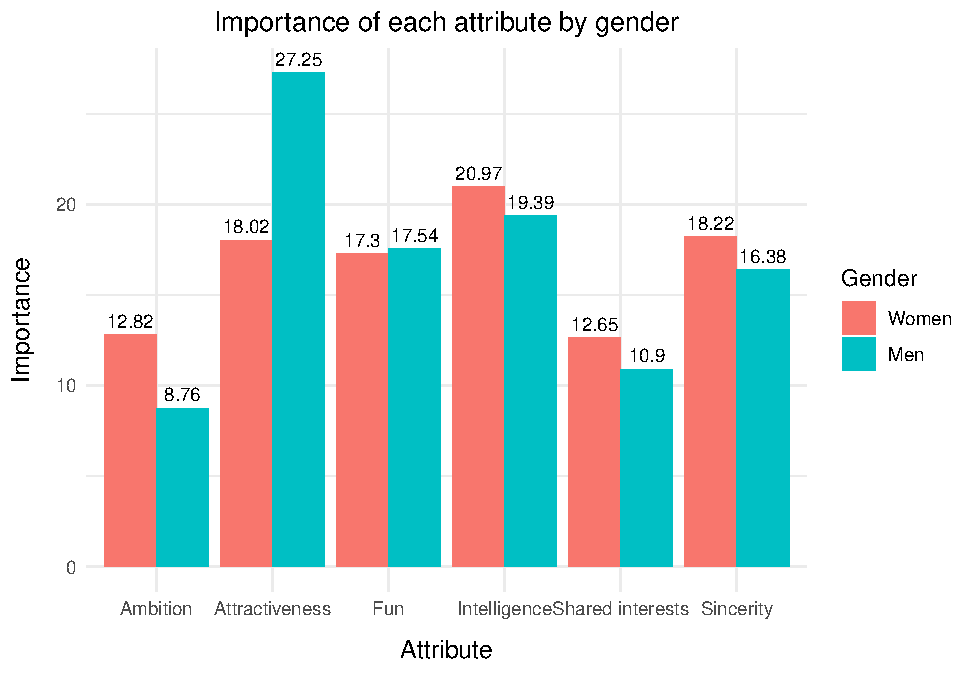
\includegraphics{SD_project_files/figure-latex/unnamed-chunk-3-1.pdf}

\begin{Shaded}
\begin{Highlighting}[]
\CommentTok{# Income}
\NormalTok{income_df <-}\StringTok{ }\KeywordTok{subset}\NormalTok{(SD, }\OperatorTok{!}\KeywordTok{duplicated}\NormalTok{(SD}\OperatorTok{$}\NormalTok{iid)) }\OperatorTok
\StringTok{  }\KeywordTok{filter}\NormalTok{(}\OperatorTok{!}\KeywordTok{is.na}\NormalTok{(income))}

\NormalTok{income_df}\OperatorTok{$}\NormalTok{gender <-}\StringTok{ }\KeywordTok{ifelse}\NormalTok{(income_df}\OperatorTok{$}\NormalTok{gender }\OperatorTok{==}\StringTok{ }\DecValTok{0}\NormalTok{, }\StringTok{'Women'}\NormalTok{, }\StringTok{'Men'}\NormalTok{)}

\NormalTok{income_df }\OperatorTok\StringTok{ }\KeywordTok{ggplot}\NormalTok{(}\KeywordTok{aes}\NormalTok{(}\DataTypeTok{x =}\NormalTok{ income}\OperatorTok{/}\DecValTok{1000}\NormalTok{, }\DataTypeTok{fill =}\NormalTok{ gender)) }\OperatorTok{+}\StringTok{ }
\StringTok{  }\KeywordTok{geom_histogram}\NormalTok{(}\DataTypeTok{bins =} \DecValTok{15}\NormalTok{)}
\end{Highlighting}
\end{Shaded}

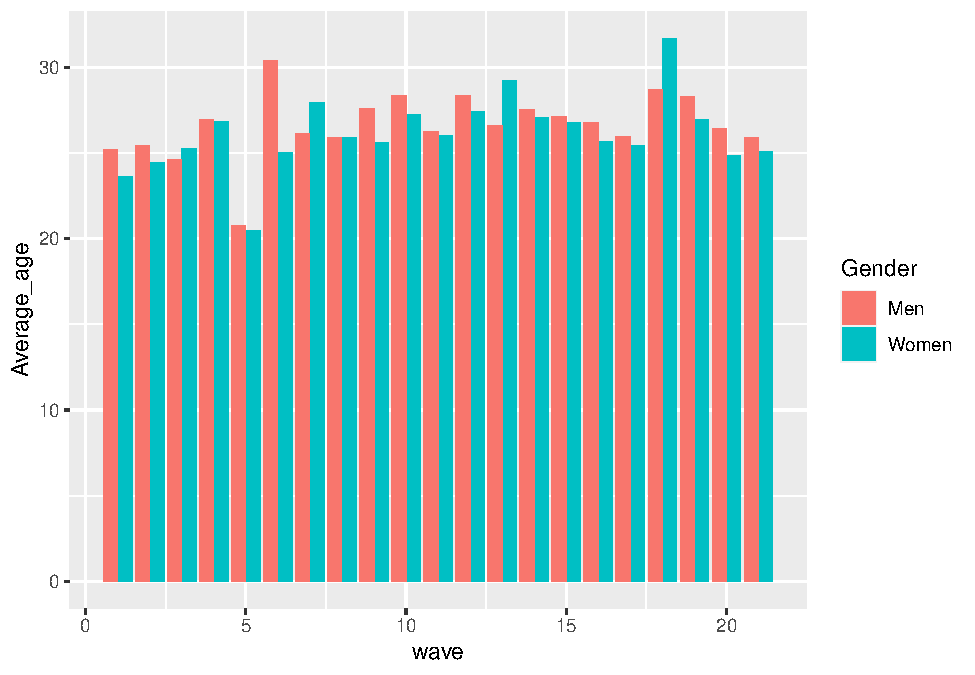
\includegraphics{SD_project_files/figure-latex/unnamed-chunk-4-1.pdf}

\begin{Shaded}
\begin{Highlighting}[]
\CommentTok{# Purpose}
\NormalTok{goal_df <-}\StringTok{ }\KeywordTok{subset}\NormalTok{(SD, }\OperatorTok{!}\KeywordTok{duplicated}\NormalTok{(SD}\OperatorTok{$}\NormalTok{iid)) }\OperatorTok
\StringTok{  }\KeywordTok{filter}\NormalTok{(}\OperatorTok{!}\KeywordTok{is.na}\NormalTok{(goal)) }\OperatorTok
\StringTok{  }\KeywordTok{group_by}\NormalTok{(goal, gender) }\OperatorTok
\StringTok{  }\KeywordTok{summarise}\NormalTok{(}\DataTypeTok{count =} \KeywordTok{n}\NormalTok{())}

\NormalTok{goal_df}\OperatorTok{$}\NormalTok{gender <-}\StringTok{ }\KeywordTok{ifelse}\NormalTok{(goal_df}\OperatorTok{$}\NormalTok{gender }\OperatorTok{==}\StringTok{ }\DecValTok{0}\NormalTok{, }\StringTok{'Women'}\NormalTok{, }\StringTok{'Men'}\NormalTok{)}

\NormalTok{goal_idx <-}\StringTok{ }\KeywordTok{unique}\NormalTok{(goal_df}\OperatorTok{$}\NormalTok{goal)}
\NormalTok{goal_val <-}\StringTok{ }\KeywordTok{c}\NormalTok{(}\StringTok{'Seemed like a fun night out'}\NormalTok{, }\StringTok{'To meet new people'}\NormalTok{, }\StringTok{'To get a date'}\NormalTok{, }
              \StringTok{'Looking for a serious relationship'}\NormalTok{, }\StringTok{'To say I did it'}\NormalTok{,  }\StringTok{'Other'}\NormalTok{)}
\NormalTok{goal_df}\OperatorTok{$}\NormalTok{goal_explained <-}\StringTok{ }\NormalTok{goal_val[}\KeywordTok{match}\NormalTok{(goal_df}\OperatorTok{$}\NormalTok{goal, goal_idx)]}

\NormalTok{goal_df }\OperatorTok\StringTok{ }\KeywordTok{ggplot}\NormalTok{(}\KeywordTok{aes}\NormalTok{(}\DataTypeTok{x =}\NormalTok{ goal_explained, }\DataTypeTok{y =}\NormalTok{ count, }\DataTypeTok{fill =}\NormalTok{ gender)) }\OperatorTok{+}\StringTok{ }
\StringTok{  }\KeywordTok{geom_bar}\NormalTok{(}\DataTypeTok{stat =} \StringTok{'identity'}\NormalTok{, }\DataTypeTok{position =} \StringTok{'dodge'}\NormalTok{) }\OperatorTok{+}
\StringTok{  }\KeywordTok{coord_flip}\NormalTok{()}
\end{Highlighting}
\end{Shaded}

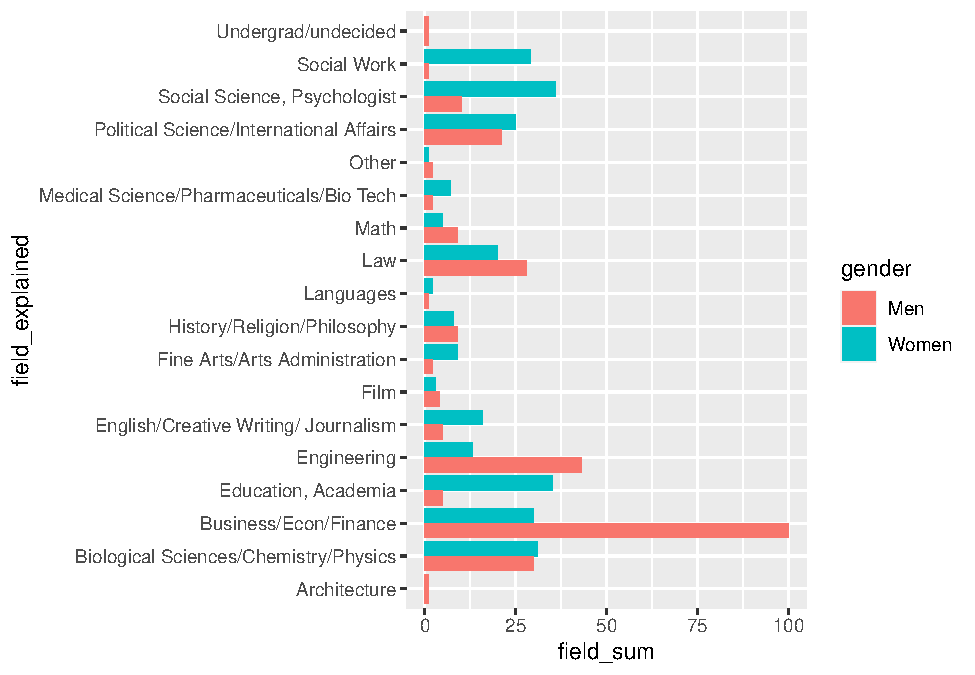
\includegraphics{SD_project_files/figure-latex/unnamed-chunk-5-1.pdf}

\begin{Shaded}
\begin{Highlighting}[]
\CommentTok{# Importance of features for men/women}
\end{Highlighting}
\end{Shaded}


\end{document}
